\section{Method}
\label{sec:method}


\noindent\begin{minipage}{\columnwidth}
\color{red}
\makeatletter
\let\draftsubsection\subsection
\def\subsection{\@startsection{subsection}{2}{\z@}{-0.10in}{0.01in}%
  {\normalsize\bf\raggedright\color{red}}}
\makeatother
\subsection{Channel Capacity Versus Denoising Steps}
\let\subsection\draftsubsection
\label{sec:channel-capacity-vs-denoising-steps}

Given a fixed computational cost $C$ in FLOPs, we profile the inference-time tradeoff between the continuous stream width $W$ and the number of denoising steps $n$ which achieve that $C$. The isoflop curves are reported in \Cref{fig:isoflop-curves}.

Using a seq2seq setup with 128 prompt tokens and 128 canvas tokens (cf. machine translation experiments in \Cref{sec:mt}), we use dummy tokens and plot the level curves for different budgets of $C$ in terms of $W$ and $n$.

\begin{center}
\captionsetup{labelfont={color=red},textfont={color=red}}
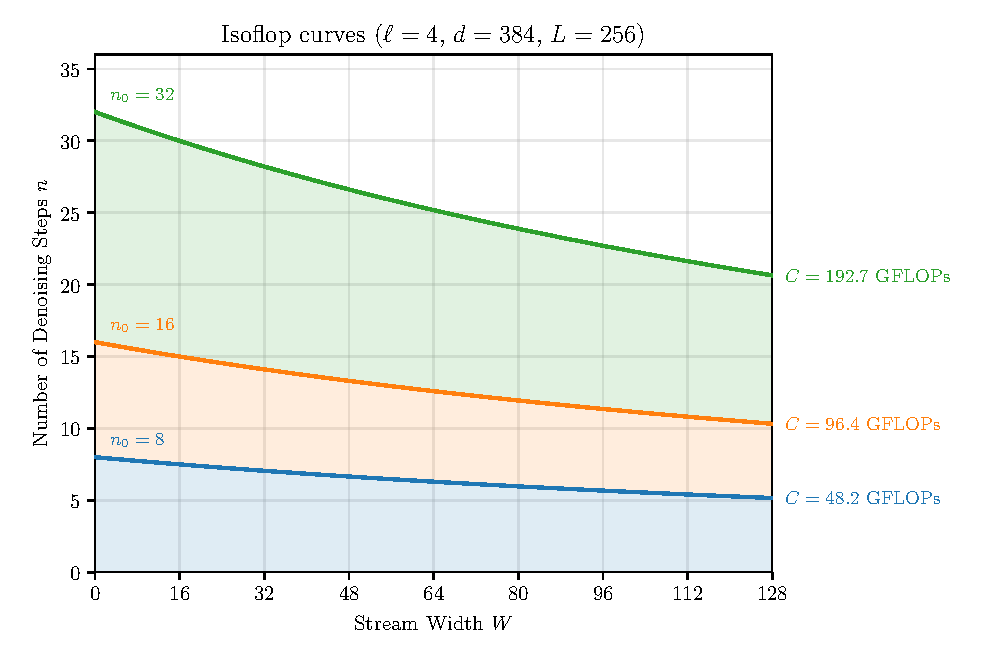
\includegraphics[width=\linewidth]{figures/isoflop_curves.pdf}
\captionof{figure}{Isoflop curves relating continuous stream width $W$ to the number of denoising steps $n$ at fixed FLOP budgets $C$.}
\label{fig:isoflop-curves}
\end{center}
\end{minipage}